
\documentclass[conference]{IEEEtran}
\IEEEoverridecommandlockouts
\usepackage{cite}
\usepackage{amsmath,amssymb}
\usepackage{graphicx}
\usepackage{booktabs}
\usepackage{array}
\usepackage{tikz}
\usetikzlibrary{arrows.meta,positioning}
\usepackage{url}

\begin{document}
\title{Transfer Learning-Based Skin Lesion Classification Using DeiT-Small on the ISIC 2019 Dataset}


\author{
\begin{minipage}[t]{0.32\textwidth}
\centering
\IEEEauthorblockN{Dr. Ankush Jain}
\IEEEauthorblockA{
Netaji Subhas University of Technology (NSUT)\\
New Delhi, India\\
ankush.jain@nsut.ac.in
}
\end{minipage}
\hfill
\begin{minipage}[t]{0.32\textwidth}
\centering
\IEEEauthorblockN{Shamayita Biswas}
\IEEEauthorblockA{
Netaji Subhas University of Technology (NSUT)\\
New Delhi, India\\
Roll No.: 2026PCS2024\\
shamayita.biswas.pg26@nsut.ac.in
}
\end{minipage}
\hfill
\begin{minipage}[t]{0.32\textwidth}
\centering
\IEEEauthorblockN{Rhydham Gundigara}
\IEEEauthorblockA{
Netaji Subhas University of Technology (NSUT)\\
New Delhi, India\\
Roll No.: 2026PCS2002\\
rhydham.gundigara.pg26@nsut.ac.in
}
\end{minipage}
}

\maketitle

\begin{abstract}
Automated skin lesion classification is challenging because dermoscopic categories exhibit visual similarities and the available images are distributed unevenly across diagnostic classes. This study investigates transfer learning for eight-class skin lesion classification using the ISIC 2019 dataset. ResNet-50 and DeiT-Small configurations were evaluated, including DeiT-Small trained with cross-entropy and class-balanced focal loss, followed by checkpoint-based fine-tuning of the selected DeiT-Small model. The final model achieved 86.19\% validation accuracy, 77.01\% balanced accuracy, 79.85\% macro F1-score, and 97.29\% macro one-versus-rest AUC on a stratified validation subset of 5,067 images. Relative to the earlier DeiT-Small cross-entropy experiment, the final fine-tuned model improved accuracy by 14.02 percentage points, balanced accuracy by 9.97 points, macro F1-score by 14.37 points, and macro-AUC by 1.97 points. Comparison with a recently published ISIC 2019 study is also provided as a cross-study reference; because the validation protocols and split sizes differ, this comparison is not interpreted as a controlled head-to-head improvement. Class-wise analysis shows the strongest recall for melanocytic nevus and lower recall for squamous cell carcinoma and actinic keratosis. The findings emphasize the importance of class-sensitive metrics and transparent comparison protocols in imbalanced medical image classification.
\end{abstract}

\begin{IEEEkeywords}
Skin lesion classification, ISIC 2019, DeiT-Small, ResNet-50, Vision Transformer, transfer learning, class imbalance, focal loss.
\end{IEEEkeywords}

\section{Introduction}
Skin cancer is an important global health concern, and timely identification of suspicious lesions can support clinical assessment and treatment planning. Dermoscopy provides magnified views of skin lesions and reveals characteristics such as pigmentation, texture, color variation, and structural patterns. Distinguishing among lesion categories remains difficult because different conditions may exhibit similar visual appearances. Deep learning has therefore been widely investigated for automated dermoscopic image classification [1], [2].

Convolutional neural networks (CNNs) learn hierarchical visual features through convolutional operations. Residual networks, in particular, use identity shortcuts to facilitate the training of deeper architectures [3]. Vision Transformers (ViTs) instead represent an image as a sequence of patches and apply self-attention to model relationships between image regions [4]. Data-efficient Image Transformers (DeiT) introduced training strategies that make transformer-based classification more data-efficient [5]. Pretrained DeiT representations can be adapted to specialized image-classification tasks through transfer learning.

The ISIC 2019 dataset contains 25,331 training dermoscopic images distributed across eight diagnostic categories: melanoma (MEL), melanocytic nevus (NV), basal cell carcinoma (BCC), actinic keratosis (AK), benign keratosis (BKL), dermatofibroma (DF), vascular lesion (VASC), and squamous cell carcinoma (SCC) [6]. Its class distribution is highly imbalanced. Consequently, overall accuracy alone may conceal poor recognition of less frequent categories. Balanced accuracy, macro F1-score, class-wise recall, and macro-AUC provide complementary views of model performance.

Loss-based methods have been proposed to mitigate imbalance. Focal loss down-weights well-classified examples and emphasizes harder samples [7], while class-balanced loss uses the effective number of samples to derive class weights [8]. Ma et al. recently investigated a ViT-based framework that combines class rebalancing with spatial- and metadata-aware feature processing [9]. Their work is used here as a literature reference, not as a directly reproduced implementation.

This paper reports a sequence of experiments on ISIC 2019 using ResNet-50 and DeiT-Small. Three earlier configurations were evaluated: ResNet-50 with cross-entropy, DeiT-Small with cross-entropy, and DeiT-Small with class-balanced focal loss and label smoothing. A subsequent checkpoint-based fine-tuning run produced the final reported DeiT-Small results. The study compares these configurations using the same four headline metrics and separately contextualizes the final result against the published reference study. The principal contributions are: (1) an empirical comparison of CNN and transformer configurations; (2) an evaluation of cross-entropy and class-balanced focal-loss training for DeiT-Small; (3) checkpoint-based fine-tuning with validation-driven selection; and (4) class-wise analysis of the final validation predictions.

\section{Related Work}
\subsection{Deep Learning for Dermoscopic Classification}
CNNs have been extensively used for skin lesion classification. Esteva et al. demonstrated the potential of deep neural networks for dermatologist-level classification of skin cancer images [1]. ResNet introduced residual learning to facilitate the optimization of deeper networks [3]. Gessert et al. studied multi-resolution EfficientNet ensembles and metadata for skin-lesion classification [10]. These studies establish the relevance of learned visual features, although differences in datasets and evaluation protocols must be considered when comparing reported scores.

\subsection{Vision Transformers}
The Vision Transformer applies transformer encoders to sequences of image patches [4]. DeiT improves the data efficiency of transformer training and provides compact model variants suitable for transfer learning [5]. In the present work, DeiT-Small is adapted to an eight-class output layer and compared with a ResNet-50 configuration.

\subsection{Learning with Imbalanced Classes}
Focal loss modifies cross-entropy by reducing the contribution of easy examples [7]. Class-balanced loss uses the effective number of samples to account for class frequency [8]. The reference study by Ma et al. combines class-balanced focal loss with additional metadata and spatial-attention components [9]. The present image-only implementation does not reproduce those additional modules; it evaluates the model configurations actually trained in this project.

\section{Proposed Methodology}
\subsection{Dataset and Data Partition}
The experiments use the 25,331-image ISIC 2019 training dataset [6]. The eight diagnostic classes are maintained in a fixed label order. The data are divided into training and validation subsets using stratified image-level sampling with a validation fraction of 0.20 and random seed 42, giving 20,264 training images and 5,067 validation images. The split is image-level and should not be described as patient-level or lesion-level partitioning.

\subsection{Preprocessing and Augmentation}
Images are converted to RGB and resized to $224\times224$ pixels. Training augmentation includes random horizontal and vertical flips, rotations up to $15^\circ$, and moderate color jitter. Images are converted to tensors and normalized using ImageNet channel means $(0.485,0.456,0.406)$ and standard deviations $(0.229,0.224,0.225)$. Validation images receive deterministic resizing and normalization without random augmentation.

\subsection{Model Configurations}
Four project configurations are included in the experimental comparison:
\begin{enumerate}
\item \textbf{ResNet-50 + cross-entropy:} a CNN baseline used to establish a reference point for the transformer experiments.
\item \textbf{DeiT-Small + cross-entropy:} a pretrained transformer with an eight-class classification head.
\item \textbf{DeiT-Small + class-balanced focal loss:} the DeiT-Small configuration trained with effective-number class weights, focal modulation, and label smoothing.
\item \textbf{Fine-tuned DeiT-Small:} the selected DeiT-Small checkpoint continued through the supplied fine-tuning pipeline. The final reported checkpoint is the cross-entropy checkpoint selected by the continuation script's default configuration.
\end{enumerate}
The final fine-tuning configuration uses AdamW, learning rate $2\times10^{-5}$, weight decay $10^{-4}$, batch size 32, maximum 10 epochs, gradient clipping at 1.0, a validation-metric-driven learning-rate scheduler, and early stopping. The best checkpoint is selected using validation macro F1-score.

\subsection{Loss Functions}
For a sample with true class $y_i$ and predicted probability $p_{i,y_i}$, cross-entropy is
\begin{equation}
L_{\mathrm{CE}}=-\frac{1}{N}\sum_{i=1}^{N}\log p_{i,y_i}.
\end{equation}
The class-balanced focal-loss experiment uses effective-number weights
\begin{equation}
E_{n_c}=\frac{1-\beta^{n_c}}{1-\beta}, \qquad
w_c=\frac{1-\beta}{1-\beta^{n_c}},
\end{equation}
where $n_c$ is the number of training examples in class $c$. The focal objective is
\begin{equation}
L_{\mathrm{CBF}}=\frac{1}{N}\sum_{i=1}^{N}
w_{y_i}(1-p_{i,y_i})^\gamma\,\mathrm{CE}_i,
\end{equation}
with effective-number parameter $\beta=0.999$, focal parameter $\gamma=2.0$, and label smoothing of 0.05 in the focal-loss configuration. The loss configuration is tied to the selected checkpoint; the final fine-tuned result is not attributed to focal loss.

\subsection{Experimental Comparison Protocol}
The four project configurations are compared using validation accuracy, balanced accuracy, macro F1-score, and macro-AUC. This table is an internal project comparison. The reference-paper results are shown separately in Section IV-C because the published study uses a different validation split and model pipeline. Any comparison with that study is therefore descriptive rather than a controlled benchmark.

\begin{figure*}[!t]
\centering
\resizebox{0.65\textwidth}{!}{%
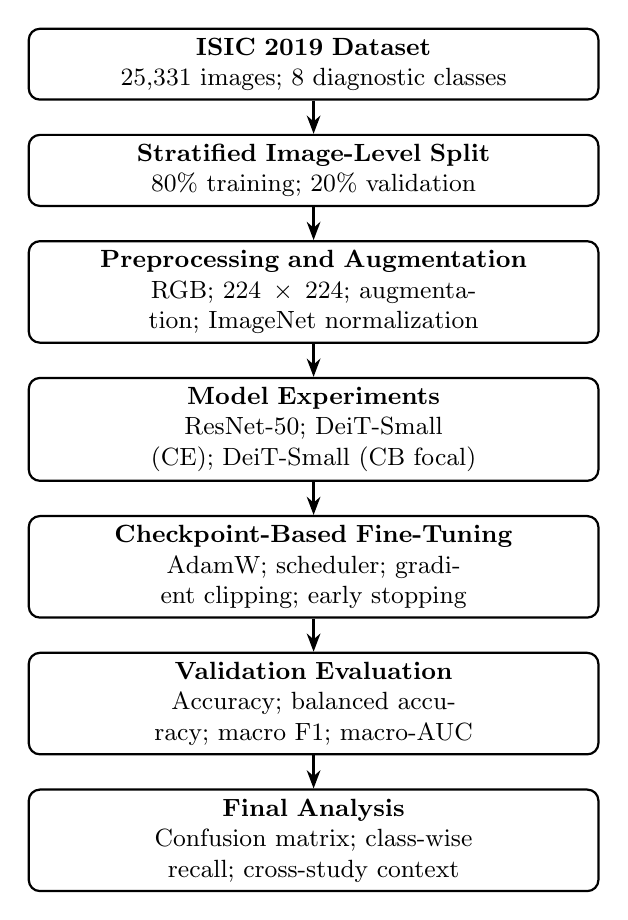
\begin{tikzpicture}[node distance=0.42cm,
block/.style={rectangle,rounded corners,draw=black,thick,text width=7cm,minimum height=0.72cm,align=center,font=\small},
arrow/.style={thick,-{Stealth}}]
\node[block] (data) {\textbf{ISIC 2019 Dataset}\\25,331 images; 8 diagnostic classes};
\node[block,below=of data] (split) {\textbf{Stratified Image-Level Split}\\80\% training; 20\% validation};
\node[block,below=of split] (prep) {\textbf{Preprocessing and Augmentation}\\RGB; $224\times224$; augmentation; ImageNet normalization};
\node[block,below=of prep] (models) {\textbf{Model Experiments}\\ResNet-50; DeiT-Small (CE); DeiT-Small (CB focal)};
\node[block,below=of models] (fine) {\textbf{Checkpoint-Based Fine-Tuning}\\AdamW; scheduler; gradient clipping; early stopping};
\node[block,below=of fine] (eval) {\textbf{Validation Evaluation}\\Accuracy; balanced accuracy; macro F1; macro-AUC};
\node[block,below=of eval] (out) {\textbf{Final Analysis}\\Confusion matrix; class-wise recall; cross-study context};
\draw[arrow] (data)--(split); \draw[arrow] (split)--(prep); \draw[arrow] (prep)--(models);
\draw[arrow] (models)--(fine); \draw[arrow] (fine)--(eval); \draw[arrow] (eval)--(out);
\end{tikzpicture}}
\caption{Experimental workflow and model-comparison pipeline.}
\label{fig:method}
\end{figure*}

\section{Experimental Setup and Results}
\subsection{Experimental Environment}
The implementation uses Python and PyTorch with the timm model library. Experiments were conducted in Google Colab. The data loader uses a batch size of 32. The validation subset contains 5,067 images. Results are reported as validation performance and not as independent test-set or clinical performance.

\subsection{Comparison of Project Models}
Table~\ref{tab:models} summarizes the model configurations evaluated during the project. The first three rows correspond to earlier model experiments; the final row is the later checkpoint-based fine-tuning result.

\begin{table*}[!t]
\caption{Internal Comparison of Evaluated Project Models on the ISIC 2019 Validation Set}
\label{tab:models}
\centering
\footnotesize
\begin{tabular}{lcccc}
\toprule
\textbf{Model Configuration} & \textbf{Accuracy (\%)} & \textbf{Balanced Acc. (\%)} & \textbf{Macro F1 (\%)} & \textbf{Macro-AUC (\%)}\\
\midrule
ResNet-50 + Cross-Entropy & 66.19 & 47.96 & 45.91 & 90.97\\
DeiT-Small + Cross-Entropy & 72.17 & 67.04 & 65.48 & 95.32\\
DeiT-Small + Class-Balanced Focal Loss & 71.72 & 70.61 & 63.86 & 94.35\\
\textbf{Fine-Tuned DeiT-Small (final)} & \textbf{86.19} & \textbf{77.01} & \textbf{79.85} & \textbf{97.29}\\
\bottomrule
\end{tabular}
\end{table*}

The initial DeiT-Small cross-entropy experiment improves over the ResNet-50 baseline by 5.98 percentage points in accuracy, 19.08 points in balanced accuracy, 19.57 points in macro F1-score, and 4.35 points in macro-AUC. The focal-loss DeiT-Small configuration yields higher balanced accuracy than the initial cross-entropy DeiT-Small run (70.61\% versus 67.04\%), while its accuracy, macro F1-score, and macro-AUC are lower. This illustrates a trade-off between aggregate accuracy and class-balanced recall rather than a uniform improvement across all metrics.

The final fine-tuned DeiT-Small model improves over the earlier DeiT-Small cross-entropy experiment by 14.02 percentage points in accuracy, 9.97 points in balanced accuracy, 14.37 points in macro F1-score, and 1.97 points in macro-AUC. Relative to the ResNet-50 experiment, the corresponding gains are 20.00, 29.05, 33.94, and 6.32 percentage points. These are absolute percentage-point differences between the recorded validation metrics; they should not be described as relative percent increases.

\subsection{Final Validation Performance}
The final fine-tuned DeiT-Small model obtains 86.19\% accuracy, 77.01\% balanced accuracy, 79.85\% macro F1-score, and 97.29\% macro-AUC. The difference between overall accuracy and balanced accuracy indicates that recall varies among diagnostic categories. Macro-AUC reflects the model's one-versus-rest ranking performance and should be interpreted alongside threshold-dependent measures.

\subsection{Contextual Comparison with the Reference Paper}
Ma et al. report an ISIC 2019 validation ablation with 3,891 images. Their baseline records 48.54\% accuracy, 90.86\% Macro-AUC, and 79.57\% Macro-BACC; their full configuration records 79.61\% accuracy, 96.13\% Macro-AUC, and 84.26\% Macro-BACC [9]. Table~\ref{tab:literature} places the final project result beside these published values.

\begin{table}[!t]
\caption{Contextual Comparison with the Published ISIC 2019 Validation Results}
\label{tab:literature}
\centering
\scriptsize
\begin{tabular}{lccc}
\toprule
\textbf{Method} & \textbf{ACC (\%)} & \textbf{Macro-AUC (\%)} & \textbf{Macro-BACC (\%)}\\
\midrule
Reference paper baseline [9] & 48.54 & 90.86 & 79.57\\
Reference paper full model [9] & 79.61 & 96.13 & 84.26\\
This work: fine-tuned DeiT-Small & 86.19 & 97.29 & 77.01\\
\bottomrule
\end{tabular}
\end{table}

Numerically, the final model is 6.58 percentage points higher in accuracy and 1.16 points higher in Macro-AUC than the reference paper's full model, while its Macro-BACC is 7.25 points lower. Compared with the reference paper's baseline row, the differences are +37.65 points in accuracy, +6.43 points in Macro-AUC, and -2.56 points in Macro-BACC. These differences must not be presented as proof that the proposed method outperforms the reference method: the reference study uses a different validation subset size (3,891 versus 5,067 images), a different architecture and training pipeline, and additional metadata/spatial modules. The table is a cross-study contextual comparison, not a same-split experiment. A defensible direct improvement claim is the within-project comparison in Table~\ref{tab:models}.

\subsection{Confusion Matrix and Class-Wise Analysis}
Fig.~\ref{fig:cm} shows the confusion matrix of the final model. The model correctly classifies 2,421 of 2,575 NV images and 571 of 665 BCC images. The most notable confusion occurs between MEL and NV: 165 MEL images are predicted as NV, while 88 NV images are predicted as MEL.

\begin{figure}[!t]
\centering
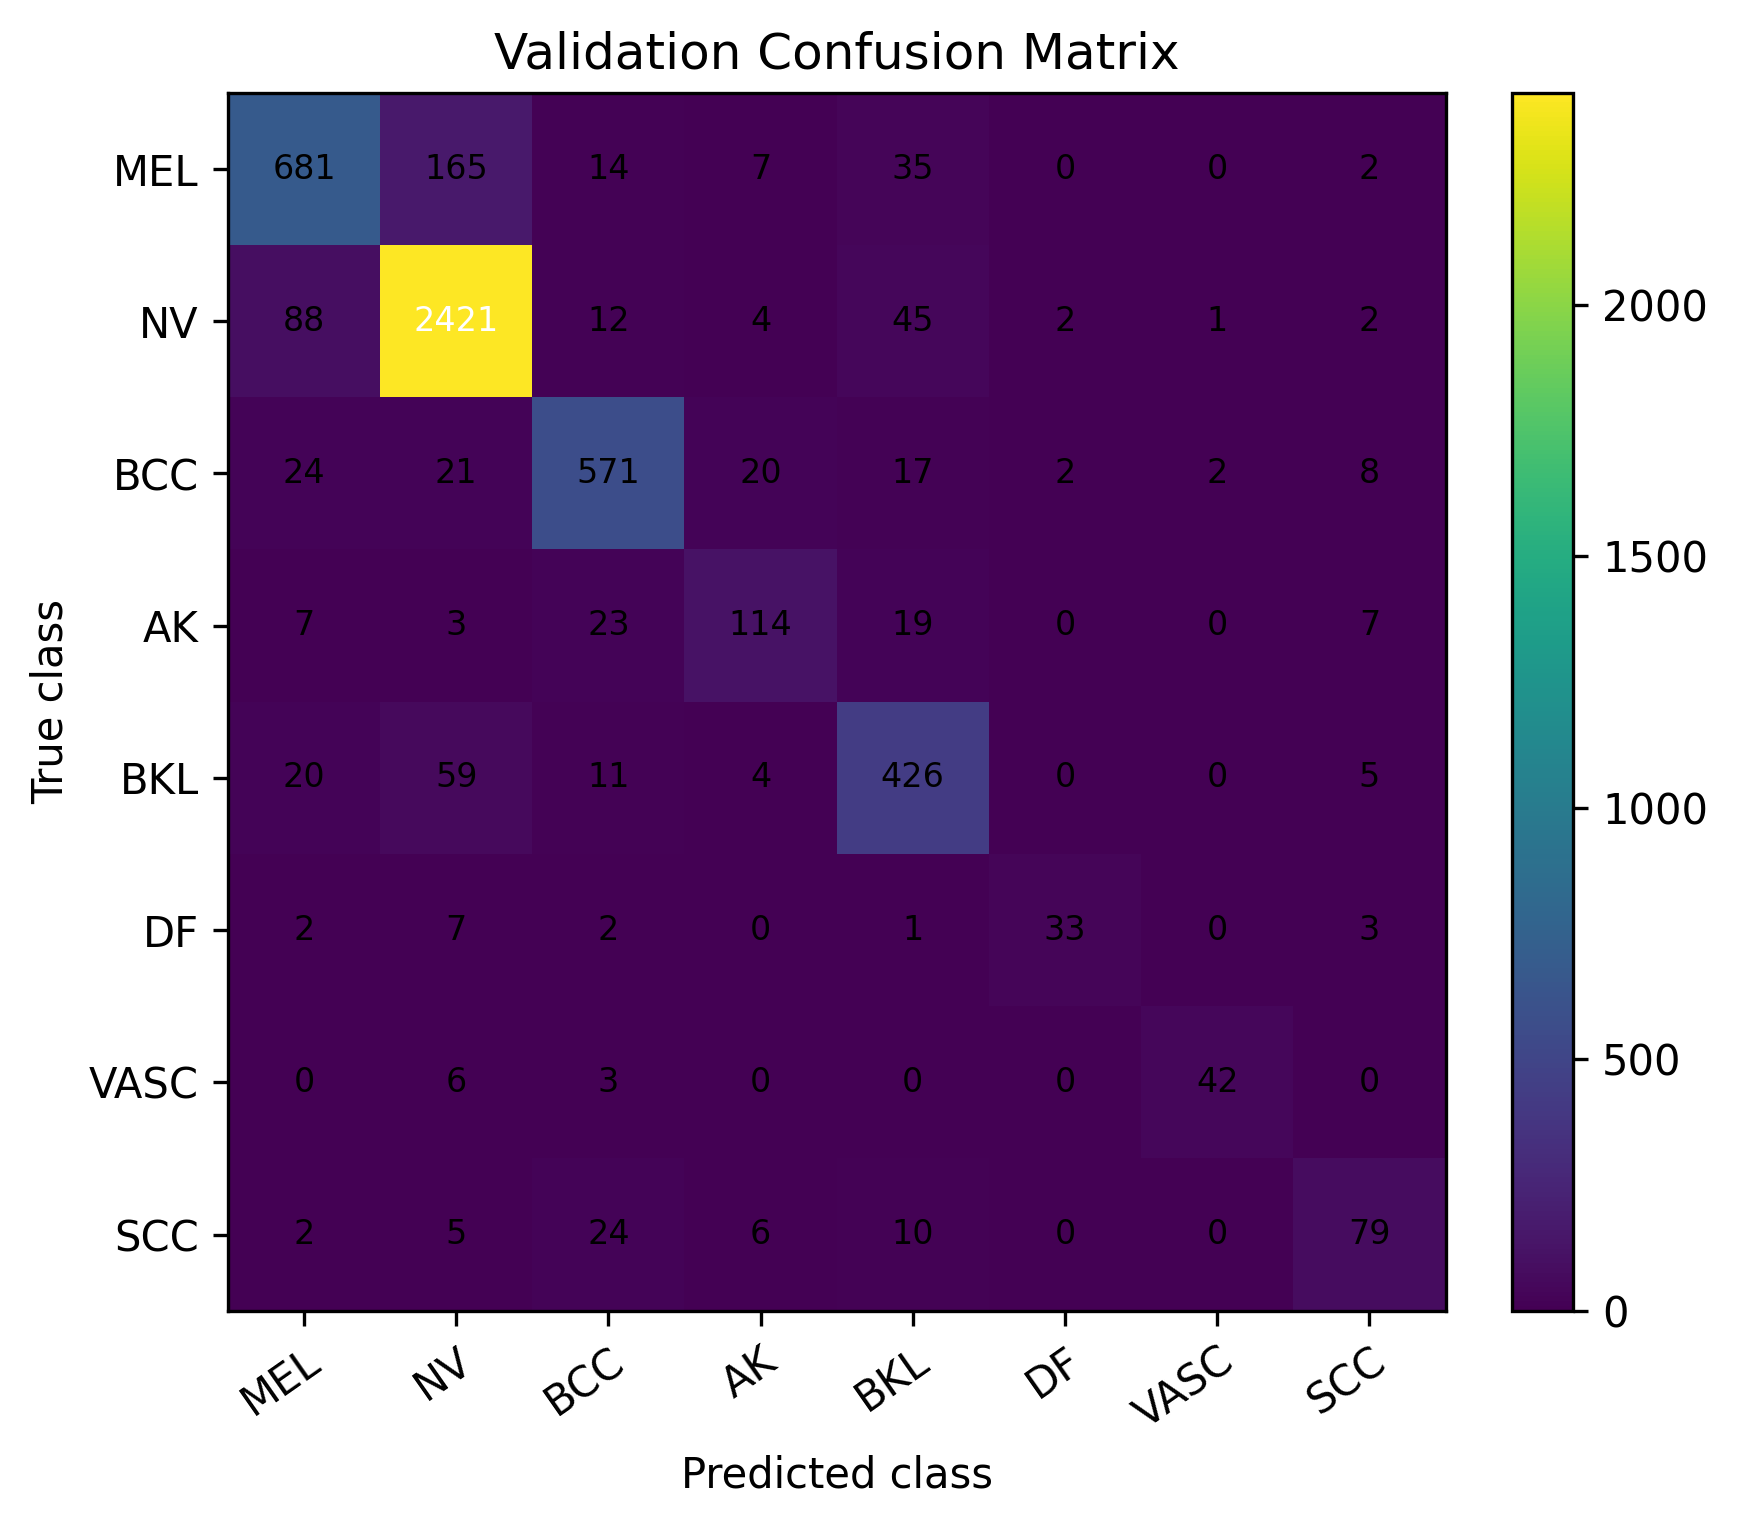
\includegraphics[width=\columnwidth]{confusion_matrix.png}
\caption{Confusion matrix of the final fine-tuned DeiT-Small model on the validation subset.}
\label{fig:cm}
\end{figure}

\begin{table}[!t]
\caption{Class-Wise Recall of the Final Model}
\label{tab:recall}
\centering
\footnotesize
\begin{tabular}{lrr}
\toprule
\textbf{Class} & \textbf{Correct/Total} & \textbf{Recall (\%)}\\
\midrule
MEL & 681/904 & 75.33\\
NV & 2421/2575 & 94.02\\
BCC & 571/665 & 85.86\\
AK & 114/173 & 65.90\\
BKL & 426/525 & 81.14\\
DF & 33/48 & 68.75\\
VASC & 42/51 & 82.35\\
SCC & 79/126 & 62.70\\
\bottomrule
\end{tabular}
\end{table}

NV achieves the highest recall at 94.02\%, followed by BCC at 85.86\%. SCC has the lowest recall at 62.70\%, followed by AK at 65.90\%. The class-wise results reinforce the importance of reporting metrics beyond overall accuracy. Recall estimates for categories with fewer validation examples, particularly DF and VASC, should be interpreted cautiously.

\subsection{Discussion and Limitations}
The internal model comparison shows that DeiT-Small outperforms the tested ResNet-50 configuration on all four recorded metrics in the earlier experiments. The focal-loss variant improves balanced accuracy over the initial DeiT-Small cross-entropy result but does not improve the other three metrics. The final fine-tuning run achieves the strongest recorded project metrics. However, the final checkpoint is the cross-entropy configuration selected by the continuation script's default setting; therefore, its performance cannot be attributed to class-balanced focal loss.

The cross-study comparison with Ma et al. is descriptive because the validation sets and methods differ. Further experiments should evaluate all architectures under an identical split and training budget, repeat runs with multiple random seeds, and include patient- or lesion-level grouping where identifiers are available. The current study uses an image-level split and does not establish external generalization or clinical readiness.

\section{Conclusion and Future Work}
This study evaluated ResNet-50 and DeiT-Small configurations for eight-class skin lesion classification using ISIC 2019. The experiments included cross-entropy training, class-balanced focal-loss training, and subsequent checkpoint-based fine-tuning. The final DeiT-Small model achieved 86.19\% accuracy, 77.01\% balanced accuracy, 79.85\% macro F1-score, and 97.29\% Macro-AUC on the 5,067-image validation subset. Compared with the earlier DeiT-Small cross-entropy experiment, the final run improved the four metrics by 14.02, 9.97, 14.37, and 1.97 percentage points, respectively. Future work will focus on controlled same-split ablations, patient/lesion-level partitioning, external validation, and analysis of lesion-focused explanations. The reported results are validation results from a research prototype and should not be interpreted as clinical diagnostic performance.

\begin{thebibliography}{00}
\bibitem{esteva2017}
A. Esteva \emph{et al.}, ``Dermatologist-level classification of skin cancer with deep neural networks,'' \emph{Nature}, vol. 542, pp. 115--118, 2017.

\bibitem{he2016}
K. He, X. Zhang, S. Ren, and J. Sun, ``Deep residual learning for image recognition,'' in \emph{Proc. IEEE Conf. Comput. Vis. Pattern Recognit. (CVPR)}, 2016, pp. 770--778.

\bibitem{dosovitskiy2021}
A. Dosovitskiy \emph{et al.}, ``An image is worth 16$\times$16 words: Transformers for image recognition at scale,'' in \emph{Proc. Int. Conf. Learn. Represent. (ICLR)}, 2021.

\bibitem{touvron2021}
H. Touvron \emph{et al.}, ``Training data-efficient image transformers \& distillation through attention,'' in \emph{Proc. Int. Conf. Mach. Learn. (ICML)}, PMLR, vol. 139, 2021, pp. 10347--10357.

\bibitem{lin2017}
T.-Y. Lin, P. Goyal, R. Girshick, K. He, and P. Doll\'ar, ``Focal loss for dense object detection,'' in \emph{Proc. IEEE Int. Conf. Comput. Vis. (ICCV)}, 2017, pp. 2980--2988.

\bibitem{isic2019}
International Skin Imaging Collaboration, ``ISIC 2019 Challenge Dataset,'' 2019. [Online]. Available: \url{https://challenge.isic-archive.com/data/}

\bibitem{cui2019}
Y. Cui, M. Jia, T.-Y. Lin, Y. Song, and S. Belongie, ``Class-balanced loss based on effective number of samples,'' in \emph{Proc. IEEE/CVF Conf. Comput. Vis. Pattern Recognit. (CVPR)}, 2019, pp. 9268--9277.

\bibitem{tschandl2018}
P. Tschandl, C. Rosendahl, and H. Kittler, ``The HAM10000 dataset, a large collection of multi-source dermatoscopic images of common pigmented skin lesions,'' \emph{Scientific Data}, vol. 5, Art. no. 180161, 2018.

\bibitem{ma2026}
T. Ma, X. Han, and G. Liu, ``Adaptive class rebalancing and spatial-aware metadata fusion for long-tailed skin lesion classification,'' \emph{Frontiers in Medicine}, vol. 13, Art. no. 1841617, 2026, doi: 10.3389/fmed.2026.1841617.

\bibitem{gessert2020}
N. Gessert \emph{et al.}, ``Skin lesion classification using ensembles of multi-resolution EfficientNets with meta data,'' \emph{MethodsX}, vol. 7, Art. no. 100864, 2020.

\bibitem{haenssle2018}
H. A. Haenssle \emph{et al.}, ``Man against machine: Diagnostic performance of a deep learning convolutional neural network for dermoscopic melanoma recognition in comparison to 58 dermatologists,'' \emph{Annals of Oncology}, vol. 29, no. 8, pp. 1836--1842, 2018.
\end{thebibliography}

\end{document}
